\documentclass[11pt]{article}
\usepackage{amsmath,textcomp,amssymb,graphicx,alltt}
\usepackage[top=1in, bottom=1in, left=.5in, right=.5in]{geometry}

\def\Name{Allen Tang, Michelle Nguyen}  % Your name

\title{CS280 -- Spring 2015 -- Homework 3}
\author{\Name}
\markboth{CS280 -- Spring 2015 Homework 3 \Name}{CS174 -- Spring 2015 Homework 3 \Name}

\pagestyle{myheadings}
\begin{document}
\maketitle

\section*{1.} We calculate F using the eight-point algorithm. Given the corresponding points in an image pair, we first normalize the points in the images to account for noise. This is done by getting the mean of the points in the first image, and subtracting that mean from those points. We also do this for the second image. We must also scale our points in the first image by $\frac{\sqrt2}{mean(x)}$, where $x$ are the distances between the newly translated points and the origin. Similarly, we do this for the second image. This gives us two transformation matrices, $T_1$ and $T_2$. We now want to find the fundamental matrix, which is given by the equation $\textbf{x}_2^tF\textbf{x}_1 = 0$. This can be written as Af = 0, where the rows of $A$ are $x_2^T x_1$ and $x_2$ and $x_1$ are normalized corresponding points. However, there is noise, so we must find an approximate solution by solving $min_f ||Af||_2$ $s.t.$ $||f||_2 = 1$. This is done by taking the right singular vector of $A$ which corresponds to the smallest singular value. However, this solution, $F*$, may not necessarily be rank 2. To assure that our fundamental matrix is of rank 2, we use SVD again. If $F*$ is $USV^t$, then $F$ is $U\hat SV^t$, where $\hat S$ is $diag(s_1, s_2, 0)$ and $s_1$ and $s_2$ are the first two diagonal elements from $S$. \\ 
We define the residual as the mean squared distance between the points in the two images and the corresponding epipolar lines. To calculate this, we first find the epipolar lines: $F\textbf{x}_1$ and $F^T\textbf{x}_2$, where the rows of $\textbf{x}_1$ and  $\textbf{x}_2$ are our original (non-transformed) homogenous points. We then find the distance of each point in the first image from its corresponding epipolar line and the distance of each point in the second image from its corresponding epipolar line. To do this, we use the distance equations, as seen below: 
\begin{verbatim}
e1_dist = (sum(e1.*[matches(:,1:2) ones(size(matches, 1), 1)], 2)./(sqrt(sum(e1(:,1:2).^2,2)))).^2
e2_dist = (sum(e2.*[matches(:,3:4) ones(size(matches, 1), 1)], 2)./(sqrt(sum(e2(:,1:2).^2,2)))).^2
\end{verbatim}
The mean of these distances is our residual error.\\
This residual is not what we are directly optimizing using SVD. By optimizing for $Af = 0$, we are trying to satisfy the constraint that our matching points lie on the epipolar plane. This does not directly mean that we are trying to minimize the distance between the points to their corresponding epipolar line. \\
For the house image, we get the fundamental matrix:
\begin{verbatim}
F =

   -0.0000    0.0000    0.0001
    0.0000   -0.0000   -0.0115
   -0.0001    0.0106   -0.0073
\end{verbatim}
This gives us a residual error of 0.0692.\\
For the library image, we get the fundamental matrix:
\begin{verbatim}
F =

   -0.0000    0.0000   -0.0001
   -0.0000   -0.0000    0.0088
    0.0011   -0.0079   -0.2140
\end{verbatim}
This gives us a residual error of 0.0575.\\
\section*{2.}
For the house image, our possible choices of t are:
\begin{verbatim}
t_1 =

   -0.9994
    0.0202
   -0.0277

t_2 =

    0.9994
   -0.0202
    0.0277
\end{verbatim}
And our possible choices of R are:
\begin{verbatim}
r_1 =

    0.9948    0.0291   -0.0980
    0.0301   -0.9995    0.0088
   -0.0977   -0.0117   -0.9951
   
r_2 =

    0.9858    0.0688   -0.1532
   -0.0702    0.9975   -0.0037
    0.1526    0.0144    0.9882
\end{verbatim}
For the library image, our possible choices of t are:
\begin{verbatim}
t_1 =

   -0.9985
    0.0048
    0.0554

t_2 =

    0.9985
   -0.0048
   -0.0554
\end{verbatim}
And our possible choices of R are:
\begin{verbatim}
r_1 =

    0.9571    0.0264   -0.2885
   -0.0257    0.9997    0.0063
    0.2886    0.0014    0.9575

r_2 =

    0.9195    0.0165   -0.3926
    0.0166   -0.9999   -0.0030
   -0.3926   -0.0037   -0.9197
\end{verbatim}

\section*{3.} We define the reconstruction error as the mean distance between the 2D points and the projected 3D points in the two images. To calculate this, after we find the 3D point for a set of corresponding points, we find the projected 3D points. We then find the distance of those corresponding points to its projected 3D point using the distance formula. A snippet of how we get the distance for a point from the first image is below:
\begin{verbatim}
sqrt((matches(n,1:1)-p1(1,:)).^2 + (matches(n,2:2)-p1(2,:)).^2)
\end{verbatim}
Finally, we get the average of all of these distances for both the first and second images, and that is our reconstruction error. \\
In this case, we are directly minimizing our reconstruction error by optimizing when solving the linear system of equations. We see that by trying to solve the equations $\textbf{x}_1 = P_1\textbf{X}$ and  $\textbf{x}_2 = P_2\textbf{X}$, we are trying to find a $\textbf{X}$ that minimizes the distance between between the projection of $\textbf{X}$ and the points $\textbf{x}_1$ and $\textbf{x}_2$, which is our reconstruction error. \\
For the house, we get a reconstruction error of 0.238478.\\
For the library, we get a reconstruction error of 0.338725.

\section*{4.}Here are some views of the house, where the green points are the camera centers:\\
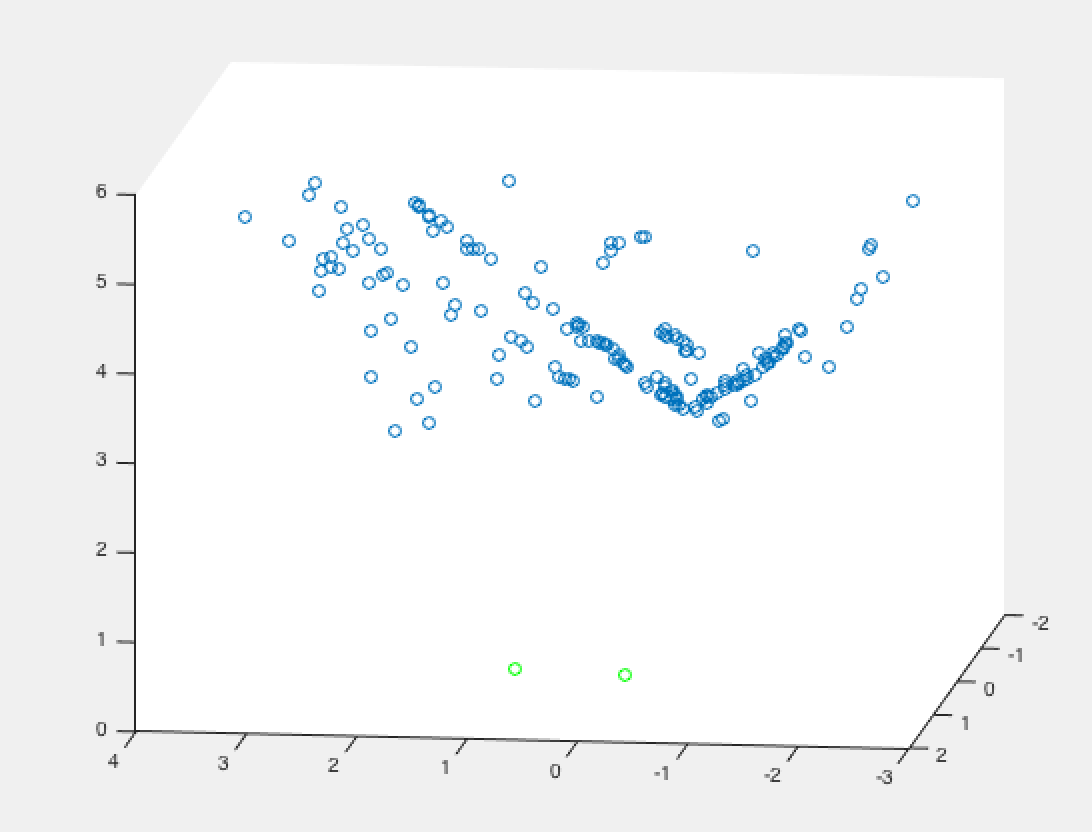
\includegraphics[scale=0.40]{house1.png} 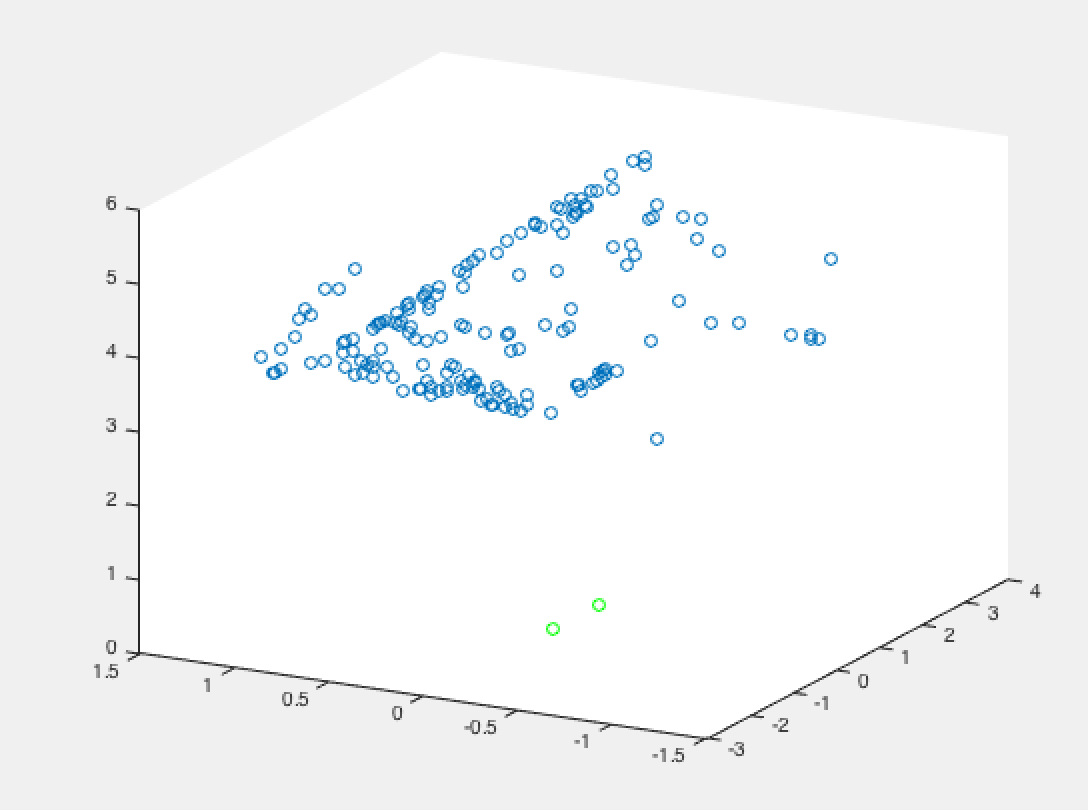
\includegraphics[scale=0.40]{house2.png}\\
Here are some views of the library, where the green points are the camera centers:\\
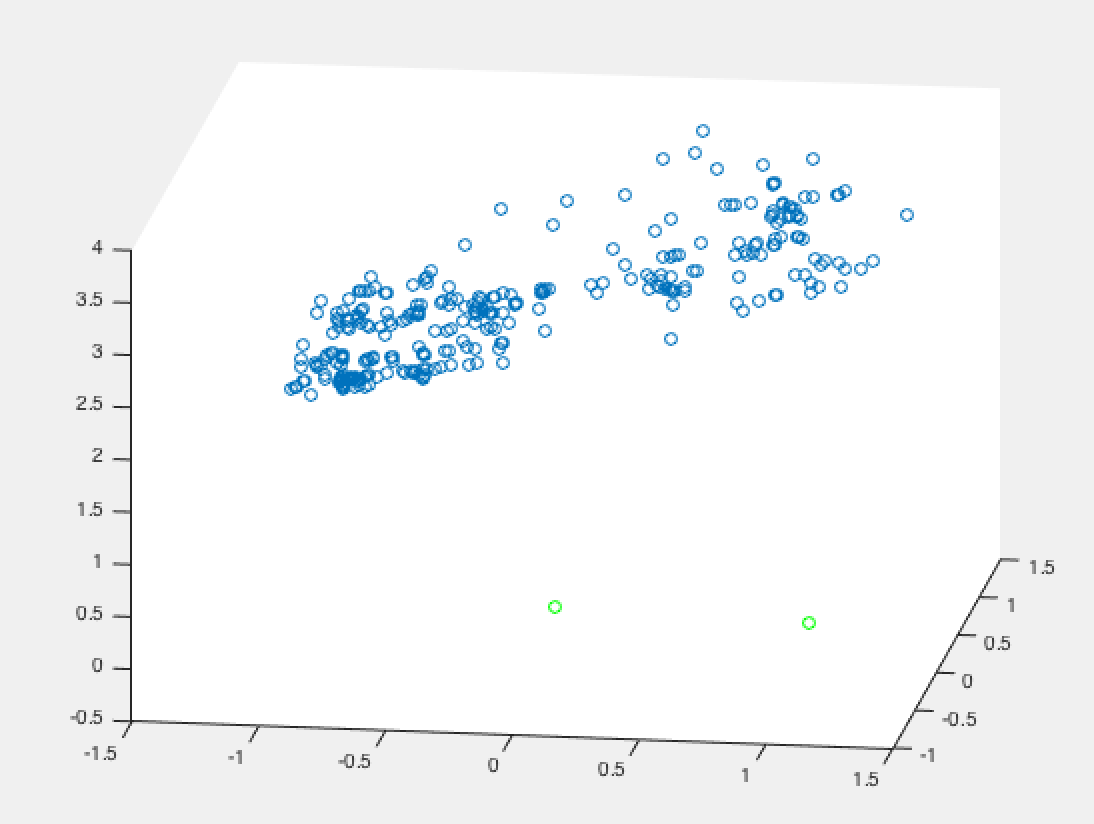
\includegraphics[scale=0.40]{library1.png} 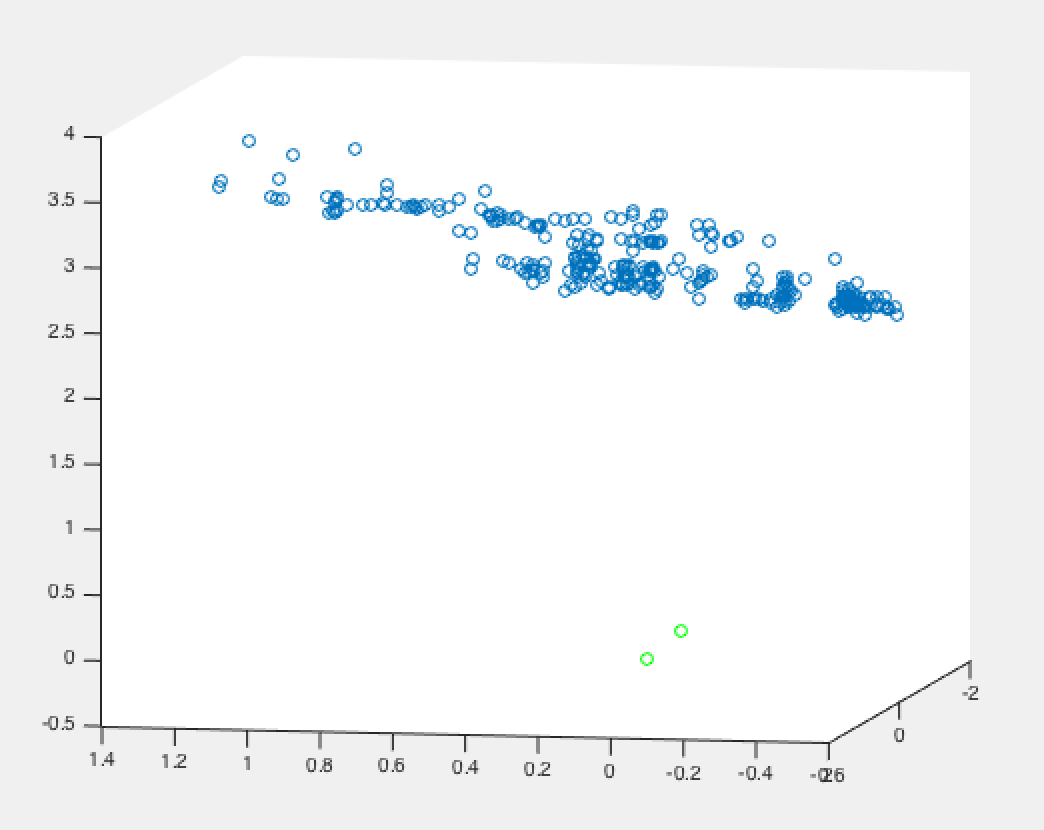
\includegraphics[scale=0.40]{library2.png}\\


\end{document}